%!TEX root = /Users/ego/Boulot/TKZ/tkz-fct/doc-fr/TKZdoc-fct-main.tex    
\section{Les différentes macros}

\tkzname{Gnuplot} détermine les points nécessaires pour tracer la courbe. Le nombre de points est fixé par l'option \tkzname{samples}; dans les premiers exemples la valeur du nombre de points est celle donnée par défaut. Ensuite  Tikz va utiliser cette table pour tracer la courbe. C'est donc \tkzname{Tikz} qui trace la courbe.

\subsection{Tracé d'une fonction avec gnuplot \tkzcname{tkzFct}}
Cette première macro est la plus importante car elle permet de tracer la représentation graphique d'une fonction continue .\hypertarget{tfct}{}

\begin{NewMacroBox}{tkzFct}{\oarg{local options}\var{gnuplot expression}} 
\emph{La fonction est donnée en utilisant la syntaxe de gnuplot. x est la variable sauf si \tkzname{xstep} est différent de 1, dans ce cas la variable est \tkzcname{x}.}

\medskip
\begin{tabular}{lll}
\toprule
 options             & exemple & explication  \\
\midrule
\TAline{gnuplot expression}{x**3}{** représente la puissance $\wedge$}
\bottomrule
\end{tabular}
 
\emph{L'expression est de la forme 2*x+1 ; 3*log(x) ; x*exp(x) ; x*x*x+x*x+x. }

Les options sont celles de \TIKZ.

\begin{tabular}{lll}
\toprule
options             & défaut & définition     \\
\midrule
\TOline{domain}{xmin:xmax}{domaine de la fonction} 
\TOline{samples}{200}{nombre de points utilisés}
\TOline{id} {tkzfct}{permet d'identifier les noms des fichiers auxiliaires}
\TOline{color}{black}{couleur de la ligne}
\TOline{line width} {1pt}{épaisseur de la ligne}
\TOline{style} {solid}{style de la ligne}
\end{tabular}
\end{NewMacroBox}

\tkzBomb Lorsque \tkzname{xstep} est différent de $1$, il est nécessaire de remplacer $x$ par |\x|.
\tkzHand Il faut bien évidemment avoir initialisé l'environnement à l'aide  \tkzcname{tkzInit} avant d'appeler \tkzcname{tkzFct}.
\tkzBomb Attention à ne pas mettre d'espace entre les arguments.   
%<--------------------------------------------------------------------------->
\subsection{option : \tkzname{samples}}

Il faut remarquer que pour tracer une droite seulement deux points sont nécessaires, ainsi le code~:

\begin{tkzltxexample}[]
\tkzFct[{-(},color=red,samples=2,domain =-1:2]{(8-1.5*\x)/2}
\end{tkzltxexample}


donne un fichier xxx.table qui contient ~:

\begin{tkzltxexample}[]
# Curve 0 of 1, 2 points
# Curve title: "(8-1.5*x)/2"
# x y type
-1.00000 4.75000  i
2.00000 2.50000  i
\end{tkzltxexample}

Ce qui est simplement suffisant. Plus simple est dans ce cas, de tracer un segment.

On demande 400 valeurs pour la table qui va permettre le tracé. Par défaut, la valeur choisie est 200.

\medskip
\begin{tkzexample}[latex=7cm]
\begin{tikzpicture}[scale=1]
    \tkzInit[xmax=5,ymax=2]
    \tkzGrid[sub]
    \tkzAxeXY
    \tkzFct[samples=400,domain=.5:5]{1/x}
\end{tikzpicture}
\end{tkzexample}

%<--------------------------------------------------------------------------->
\subsection{options : \tkzname{xstep, ystep}}


\begin{tkzexample}[]
\begin{tikzpicture}
\tkzInit[xmax= 110,xstep=10,
         ymax=6,ystep=1]
\tkzDrawX[label={\textit{Age}},below= -18pt]
\tkzLabelX
\tkzDrawY[label={\textit{litres}}]
\tkzFct[domain = 0.1:100 ]{50/\x}
\end{tikzpicture} 
\end{tkzexample}


\subsection{Modification de \tkzname{xstep} et \tkzname{ystep}}

Cette fois le domaine s'étend de 0 à 800, les valeurs prises par la fonction de $0$ à $\numprint{2000}$. \tkzname{xstep=100} donc il faut utiliser |\x| à la place de $x$. Une petite astuce au niveau de gnuplot, 1. et 113. permettent d'obtenir une division dans les décimaux sinon la division se fait dans les entiers.

Ensuite, j'utilise les macros pour placer des points
%<--------------------------------------------------------------------------->
\begin{tkzexample}[vbox]
\begin{tikzpicture}[scale=1.5]
 \tkzInit[xmax=700,xstep=100,ymax=1200,ystep=400]
 \tkzGrid(0,0)(700,1200)  \tkzAxeXY
 \tkzFct[color=red,samples=100,line width=0.8pt,domain =0:700]%
        {(1./90000)*\x*\x*\x-(1./100)*\x*\x+(113./36)*\x}
\end{tikzpicture}
\end{tkzexample}

\subsection{\tkzname{ystep} et les fonctions constantes}

Attention, ici  \tkzname{ystep=6} or \tkzname{gnuplot} donne $80\div=13$. il faut donc écrire $80.$

\begin{tkzexample}[vbox]
 \begin{tikzpicture}[scale=0.4]
 \tkzInit[xmax=30,ymax=90,ystep=6]
 \tkzAxeX[nograd,noticks,poslabel=right,label=$t$] 
 \tkzAxeY[nograd,noticks,poslabel=above,label=$P$] 
 \tkzFct[line width=1pt,color=red,dashed,domain=0:30]{80.0}
 \tkzFct[line width=1pt,color=blue,domain=0:30]{80/(1.0+4.0*exp(-0.21*x))}
 \tkzText[above,color=red](20,80){$P=80$}
\end{tikzpicture}  
\end{tkzexample}

\subsection{Les fonctions affines ou linéaires}
Pour obtenir des droites, on peut utiliser \tkzname{gnuplot} même si l'outil est un peu lourd dans ce cas. Pour alléger les calculs, il est possible de ne demander que deux points !

\begin{tkzexample}[vbox]
 \begin{tikzpicture}[]
 \tkzInit[ymax=20,ystep=5]
 \tkzAxeXY
 \tkzFct[color=red,domain=0:10,samples=2]{2*x+5}
 \tkzFct[color=blue,domain=0:10,samples=2]{-x+15}
 \tkzFct[color=green,domain=0:10,samples=2]{7} % 7/5=1
 \tkzFct[color=purple,domain=0:10,samples=2]{7.}%7.0/5 =1.2  
\end{tikzpicture}   
\end{tkzexample}
   %<--------------------------------------------------------------------------->
\subsection{Sous-grille}
 
   $y=(x-4)\text{e}^{-0.25x+5}$

Il est possible de dessiner une autre grille.

\begin{tkzexample}[latex=8cm]
\begin{tikzpicture}
 \tkzInit[xmin=4,xmax=18,xstep=2,
          ymin=20,ymax=90,ystep=10]
 \tkzFct[domain = 5:18]%
        {(\x-4)*exp(-0.25*\x+5)}
 \tkzGrid(4,20)(18,90)
 \tkzAxeXY
 \tkzGrid[sub,
          subxstep=0.5,
          subystep=2,
          color=brown](6,60)(12,90)
\end{tikzpicture}
\end{tkzexample}
%<--------------------------------------------------------------------------->
\subsection{Utilisation des macros de \tkzname{tkz-base}}
Toutes les macros de  \tkzname{tkz-base} sont bien sûr utilisables, en voici quelques exemples.

\begin{center}
	\begin{tkzexample}[vbox]
	\begin{tikzpicture}[scale=2]
	 \tkzInit[xmin=-3,xmax=3, ymin=-1,ymax=3]
	 \tkzGrid[sub,subxstep=.5,subystep=.5]
	 \tkzAxeXY
	 \tkzFct[domain = -3:2]{(2-x)*exp(x)}
	 \tkzText(-2,1.25){$\mathcal{C}_{f}$}
	 \tkzDefPoint(2,0){A} \tkzDrawPoint(A)  \tkzLabelPoints(A)
	 \end{tikzpicture}
	\end{tkzexample}  
\end{center}

  
%<--------------------------------------------------------------------------->
\endinput
